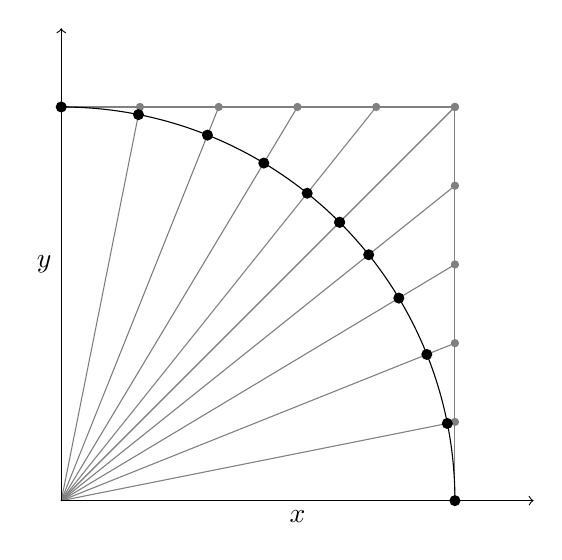
\begin{tikzpicture}

    \draw[gray] (5,0) -- (5,5);
    \draw[gray] (0,5) -- (5,5);

    \foreach \x in {0,1,2,3,4,5} {
        \draw[gray] (\x,5) -- (0,0);    
        \draw[gray] (5,\x) -- (0,0);    
        \fill[gray] (\x,5) circle (1.5pt);
        \fill[gray] (5,\x) circle (1.5pt);

        \pgfmathsetmacro{\r}{sqrt(\x*\x + 25)}
        \pgfmathsetmacro{\projx}{\x / \r * 5}
        \pgfmathsetmacro{\projy}{5 / \r * 5}

        \fill (\projx,\projy) circle (2pt);
        \fill (\projy,\projx) circle (2pt); 
    }

    \draw (5,0) arc[start angle=0, end angle=90, radius=5];    

    % Draw axes
    \draw[->] (0,0) -- (6,0) node[midway, below] {\( x \)};
    \draw[->] (0,0) -- (0,6) node[midway, left] {\( y \)};
\end{tikzpicture}
